\documentclass[dvipdfmx,cjk,xcolor=dvipsnames,envcountsect,notheorems,12pt]{beamer}
% * 16:9 のスライドを作るときは,aspectratio=169 を documentclass のオプションに追加する
% * 印刷用の配布資料を作るときは handout を documentclass のオプションに追加する
% (overlay が全て一つのスライドに出力される)

\usepackage{pxjahyper}% しおりの文字化け対策 (なくても良い)
\usepackage{amsmath,amssymb,amsfonts,amsthm,ascmac,cases,bm,pifont}
\usepackage{graphicx}
\usepackage{url}

\usepackage{proof}
% \usepackage{tikz}
% \usetikzlibrary{positioning}

\newcommand\fun[2]{\lambda{#1}.{#2}}

\newcommand\Resetz{\textbf{reset0}}
\newcommand\Shiftz{\textbf{shift0}}
\newcommand\Throw{\textbf{throw}}
\newcommand\resetz[1]{\Resetz~{#1}}
\newcommand\shiftz[2]{\Shiftz~{#1}.{#2}}
\newcommand\throw[2]{\Throw~{#1}~{#2}}

\newcommand\cfun[2]{\underline{\lambda}{#1}.{#2}}

\newcommand\cResetz{\underline{\textbf{reset0}}}
\newcommand\cShiftz{\underline{\textbf{shift0}}}
\newcommand\cThrow{\underline{\textbf{throw}}}
\newcommand\cresetz[1]{\cResetz~{#1}}
\newcommand\cshiftz[2]{\cShiftz~{#1}\to{#2}}
\newcommand\cthrow[2]{\cThrow~{#1}~{#2}}

\newcommand\cPlus{\underline{\textbf{+}}}

\newcommand\cLet{\underline{\textbf{clet}}}
\newcommand\cIn{\underline{\textbf{in}}}
\newcommand\clet[3]{\cLet~{#1}={#2}~\cIn~{#3}}
\newcommand\csp[1]{\texttt{\%}{#1}}
\newcommand\code[1]{\texttt{<}{#1}\texttt{>}}

\newcommand\codeT[2]{\langle{#1}\rangle^{#2}}
\newcommand\contT[2]{({#1} \Rightarrow {#2})}

\newcommand\ord{\ge}

\newcommand\too{\leadsto^*}
\newcommand\pink[1]{\textcolor{pink}{#1}}
\newcommand\red[1]{\textcolor{red}{#1}}
\newcommand\green[1]{\textcolor{green}{#1}}
\newcommand\magenta[1]{\textcolor{magenta}{#1}}
\newcommand\blue[1]{\textcolor{blue}{#1}}

% スライドのテーマ
\usetheme{sumiilab}
% ベースになる色を指定できる
% \usecolortheme[named=Magenta]{structure}
% 数式の文字が細くて見難い時は serif の代わりに bold にしましょう
% \mathversion{bold}

%% ===============================================
%% スライドの表紙および PDF に表示される情報
%% ===============================================

%% 発表会の名前とか(省略可)
% \session{研究室ゼミ}
%% スライドのタイトル
% \title{多段階 let 挿入を行うコード生成言語の設計}
\title{多段階let 挿入を行うコード生成言語の設計}
%% 必要ならば,サブタイトルも
% \subtitle{}
%% 発表者のお名前
\author{大石純平}
%% 発表者の所属([] 内は短い名前)
% \institute[東北大学 住井・松田研]{東北大学 工学部 電気情報物理工学科\\住井・松田研究室}% 学部生
\institute[筑波大学 プログラム論理研究室]{筑波大学 大学院 \\ プログラム論理研究室}% 院生
%% 発表する日
\date{2016/7/12}

%% ===============================================
%% 自動挿入される目次ページの設定(削除しても可)
%% ===============================================

% section の先頭に自動挿入される目次ページ(削除すると,表示されなくなる)
\AtBeginSection[]{
  \begin{frame}
    \frametitle{アウトライン}
    \tableofcontents[sectionstyle=show/shaded,subsectionstyle=show/show/hide]
  \end{frame}}
% subsection の先頭に自動挿入される目次ページ(削除すると,表示されなくなる)
% \AtBeginSubsection[]{
%   \begin{frame}
%     \frametitle{アウトライン}
%     \tableofcontents[sectionstyle=show/shaded,subsectionstyle=show/shaded/hide]
%   \end{frame}}

%% 現在の section 以外を非表示にする場合は以下のようにする

%% \AtBeginSection[]{
%% \begin{frame}
%%   \frametitle{アウトライン}
%%   \tableofcontents[sectionstyle=show/hide,subsectionstyle=show/show/hide]
%% \end{frame}}
%% \AtBeginSubsection[]{
%% \begin{frame}
%%   \frametitle{アウトライン}
%%   \tableofcontents[sectionstyle=show/hide,subsectionstyle=show/shaded/hide]
%% \end{frame}}

%% ===============================================
%% 定理環境の設定
%% ===============================================

\setbeamertemplate{theorems}[numbered]% 定理環境に番号を付ける
\theoremstyle{definition}
\newtheorem{definition}{定義}
\newtheorem{axiom}{公理}
\newtheorem{theorem}{定理}
\newtheorem{lemma}{補題}
\newtheorem{corollary}{系}
\newtheorem{proposition}{命題}

%% ===============================================
%% ソースコードの設定
%% ===============================================

\usepackage{listings,jlisting}
% \usepackage[scale=0.9]{DejaVuSansMono}

\definecolor{DarkGreen}{rgb}{0,0.5,0}
% プログラミング言語と表示するフォント等の設定
\lstset{
  language={[Objective]Caml},% プログラミング言語
  basicstyle={\ttfamily\small},% ソースコードのテキストのスタイル
  keywordstyle={\bfseries},% 予約語等のキーワードのスタイル
  commentstyle={},% コメントのスタイル
  stringstyle={},% 文字列のスタイル
  frame=trlb,% ソースコードの枠線の設定 (none だと非表示)
  numbers=none,% 行番号の表示 (left だと左に表示)
  numberstyle={},% 行番号のスタイル
  xleftmargin=5pt,% 左余白
  xrightmargin=5pt,% 右余白
  keepspaces=true,% 空白を表示する
  mathescape,% $ で囲った部分を数式として表示する ($ がソースコード中で使えなくなるので注意)
  % 手動強調表示の設定
  moredelim=[is][\itshape]{@/}{/@},
  moredelim=[is][\color{red}]{@r\{}{\}@},
  moredelim=[is][\color{blue}]{@b\{}{\}@},
  moredelim=[is][\color{DarkGreen}]{@g\{}{\}@},
  moredelim=[is][\color{Magenta}]{@m\{}{\}@},
}

%% ===============================================
%% 本文
%% ===============================================
\begin{document}
\frame[plain]{\titlepage}% タイトルページ

\section*{アウトライン}

% 目次を表示させる(section を表示し,subsection は隠す)
\begin{frame}
  \frametitle{アウトライン}
  \tableofcontents[sectionstyle=show,subsectionstyle=hide]
\end{frame}

\section{概要}
\begin{frame}
  \frametitle{概要}
  \begin{itemize}
  \item Sudo らが作ったコード体系の型システムでは,
    \alert{破壊的代入}という副作用を扱うようなコード生成の安全性を保証した.
  \item しかし,\alert{多段階のlet 挿入}を扱うようなコード生成の安全性は保証していなかった
  \item[⇒] \alert{多段階のlet挿入}を安全に扱うために型システムを改良した.
  \end{itemize}
\end{frame}

\section{研究の背景}
\subsection{段階的計算(コード生成)}
\begin{frame}
  \frametitle{段階的計算 (Staged Computation)}
  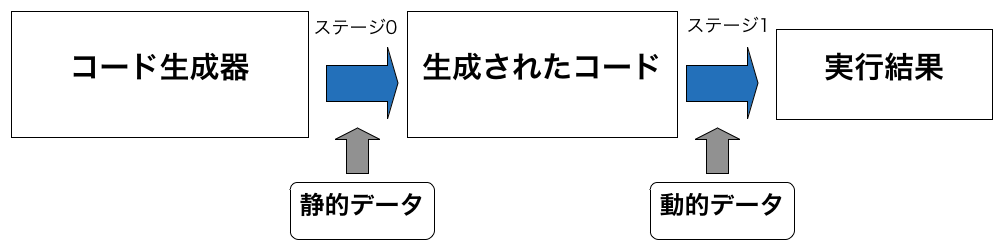
\includegraphics[clip,width=12cm]{./img/prggen.png}

  \begin{itemize}
  \item コード生成ステージとコード実行ステージ
  \item 「保守性・再利用性の高さ」と「実行性能の高さ」の両立
  \item[⇒] 段階的計算をサポートするプログラム言語 ⇒ コード生成言語
    % \item 生成するプログラムだけでなく,生成されたプログラムも型の整合性が静的に (生成前に) 保証される.
  \end{itemize}
\end{frame}

\subsection{コード生成の例}
\begin{frame}
  \frametitle{power関数のコード化}
  \begin{align*}
    \text{power} ~x~ ~n~ &~=~ x &\text{if} ~~n = 1 \\
                         &~~~\phantom{=}~ x * \text{power}(x, n-1) &\text{if} ~~n > 1
  \end{align*}

  \pause
  8に特化したコードの生成を行う
  \begin{align*}
    \text{gen\_power} ~x~ ~8~ =~ ~x~ * ~x~ * ~x~ * ~x~ * ~x~ * ~x~ * ~x~ * ~x~
  \end{align*}
  \pause
  $\text{gen\_power} ~x~ ~8~$ は$\text{power} ~x~ ~8~$ より高速
  \begin{itemize}
  \item 関数呼び出しがない
  \item 条件式がない
  \end{itemize}
\end{frame}

\subsection{段階的計算の課題}

\begin{frame}
  \frametitle{コード生成における課題}
  % もっとコンパクトに
  生成されたコードの信頼性(正しさ)
  \begin{itemize}
  \item パラメータに応じて,非常に多数のコードが生成される
    % \item 構文的,意味的に正しくないプログラムを生成しやすい
  \item 生成したコードのデバッグが容易ではない
  \item [⇒]コード生成の前に安全性を保証したい
  \end{itemize}

  \uncover<2->{従来研究}
  \begin{itemize}
  \item<2-> コード生成プログラムが,安全なコードのみを生成する事を保証
    % \item<2-> let挿入等を実現する\alert{計算エフェクトを含む場合の安全性保証の研究は未整備}
  \item<3-> 安全なコード: 構文,型,変数束縛が正しいプログラム
  \item<4-> \alert{let挿入}等を実現する\alert{計算エフェクトを含む場合の安全性保証は研究途上}
  \end{itemize}
\end{frame}

\subsection{限定継続}

\begin{frame}
  \frametitle{コントロールオペレータ}
  \begin{block}{プログラミング言語におけるプログラムを制御するプリミティブ}
    \begin{itemize}
    \item exception (例外): C++, Java, ML
    \item call/cc (第一級継続): Scheme, SML/NJ
    \item shift/reset (限定継続): Racket, Scala, OCaml
      \begin{itemize}
      \item 1989年以降多数研究がある
      \item コード生成におけるlet挿入が実現可能
        % \item shift/reset + コード生成の型システムが幾つか提案されている
      \end{itemize}
    \item \alert{shift0/reset0}
      \begin{itemize}
        \item 2011年以降研究が活発化.
        \item コード生成における\alert{多段階let挿入}が可能
      \end{itemize}
    \end{itemize}
  \end{block}
\end{frame}

% \begin{frame}
%   \frametitle{shift0 / reset0}
%   % \begin{align*}
%   %   (\cResetz ~...~ (\cShiftz ~k \to ~e~) ~...~)
%   % \end{align*}

%   % \begin{onlyenv}<1>
%   %   \begin{align*}
%   %     5 ~*~ (\cResetz ~3 ~+~ (\cShiftz ~k \to ~k ~4))
%   %   \end{align*}
%   % \end{onlyenv}

%   % \begin{onlyenv}<2>
%   %   \begin{align*}
%   %     5 * \cResetz 1 + (\cShiftz ~k \to k 1)
%   %   \end{align*}
%   % \end{onlyenv}

% \end{frame}

% \subsection{コントロールオペレータ}

% \begin{frame}[fragile]
%   \frametitle{shift0/reset0とshift/reset}
%   %   shift0/reset0はshift/reset とほぼ同様な計算規則で定義されている.その差は僅かです
%   %   しかし shiftは直近のresetまでのプログラムの部分を切り取ることができますが,それ以上の2番目3番目のresetまでのプログラムの部分を切り取ることはできません.
%   %   一方でMaterzokらによってshift0をうまく使うことによって直近のshift0だけでなく,2番目3番目のreset0までのプログラムの部分を切り取ることができることがわかっています.

%   %   このような働きを持つオペレータはコード生成に非常に有用であることに着目してこの研究をはじめました.Materzokらはラムダ計算に対してshift0/reset0の性質を解明したのですが,本研究ではこれをコード生成言語の多段階let挿入に使えることを思いつき,そのような体系を作りたいというのが本研究の基本着想です.

%   shift0/reset0とshift/resetはわずかに異なる

%   %   より簡潔なCPSの意味論をもち,
%   %   それでいて,表現力は階層的shift/resetを完全に表現できる.(例えば多段階let挿入が可能)
%   %   ごく最近2011年以降研究されている.
%   \begin{center}
%     shift0/reset0: $\langle K [S_0 f.e] \rangle \rightsquigarrow e \{ f / \lambda x . \langle K [x] \rangle \}$\\
%     shift/reset:  \,\,\,\,$\langle K [S f.e] \rangle \rightsquigarrow \langle e \{ f / \lambda x . \langle K [x] \rangle \} \rangle $
%   \end{center}

%   %   shift0は,直近のreset0より,遠くのreset0までアクセスできる.
%   \begin{columns}
%     \begin{column}{.5\textwidth}
%       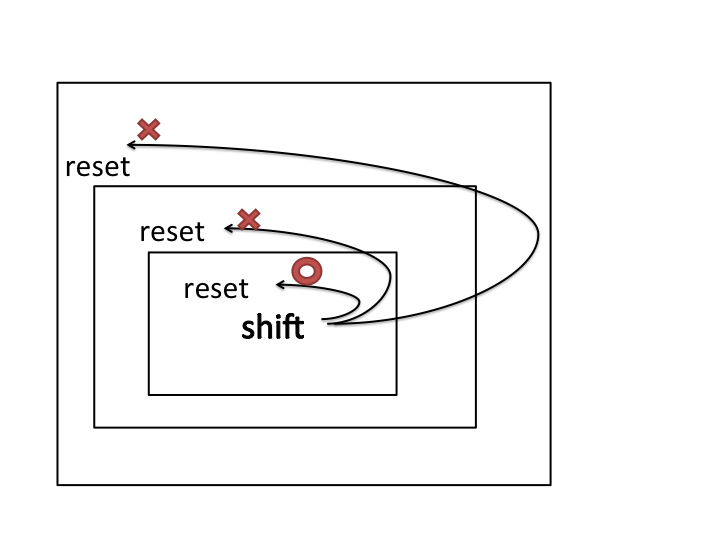
\includegraphics[clip,width=8cm]{./img/sr.png}
%     \end{column}

%     \begin{column}{.5\textwidth}
%       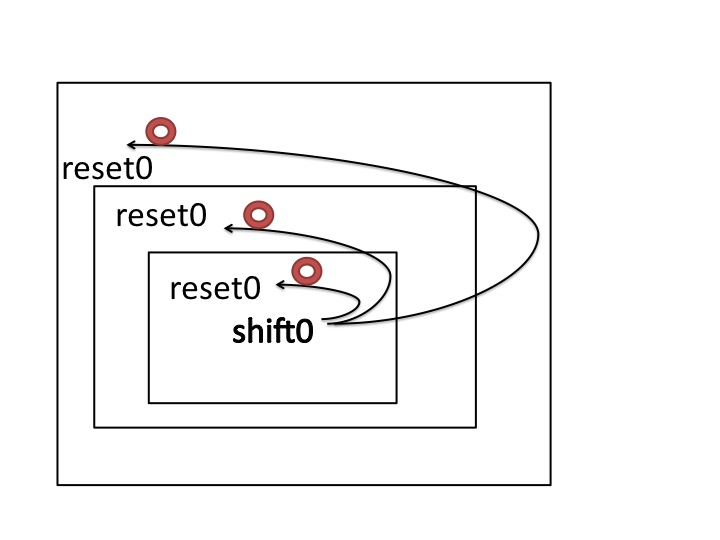
\includegraphics[clip,width=8cm]{./img/s0r0.png}
%     \end{column}
%   \end{columns}

% \end{frame}

\subsection{shift0/reset0}

\begin{frame}[fragile]
  \frametitle{多段階let 挿入}
  \begin{align*}
    & \cLet~x_1=\csp{3}~\cIn \\
    & \cLet~x_2=\csp{5}~\cIn \\
    & \magenta{\cLet~y=t~\cIn} \\
    & (x_1~\cPlus~x_2~\cPlus~y)
  \end{align*}

  \pause

  \begin{align*}
    & \red{\cResetz} ~~\cLet~x_1=\csp{3}~\cIn \\
    & \blue{\cResetz} ~~\cLet~x_2=\csp{5}~\cIn \\
    & \blue{\cShiftz}~\blue{k_2}~\to~ \red{\cShiftz}~\red{k_1}~\to~ \magenta{\cLet~y=t~\cIn} \\
    & \red{k_1}~(~\blue{k_2}~(x_1~\cPlus~x_2~\cPlus~y))
  \end{align*}
\end{frame}

\begin{frame}[fragile]
  \frametitle{多段階let 挿入}
  \begin{onlyenv}<1>
    \begin{align*}
      & \red{\cResetz} ~~\cLet~x_1=\csp{3}~\cIn \\
      & \blue{\cResetz} ~~\cLet~x_2=\csp{5}~\cIn \\
      & \blue{\cShiftz}~\blue{k_2}~\to~ \red{\cShiftz}~\red{k_1}~\to~ \magenta{\cLet~y=t~\cIn} \\
      & \red{k_1}~(~\blue{k_2}~(x_1~\cPlus~x_2~\cPlus~y))
    \end{align*}
  \end{onlyenv}

  \begin{onlyenv}<2>
    \begin{align*}
      & \magenta{\cLet~y=t~\cIn} \\
      & \cLet~x_1=\csp{3}~\cIn \\
      & \cLet~x_2=\csp{5}~\cIn \\
      & (x_1~\cPlus~x_2~\cPlus~y)
    \end{align*}
  \end{onlyenv}
\end{frame}

\begin{frame}
  \frametitle{多段階let挿入の結果}
  \begin{align*}
    & \cLet~x_1=\csp{3}~\cIn \\
    & \cLet~x_2=\csp{5}~\cIn \\
    & \magenta{\cLet~y=t~\cIn} \\
    & (x_1~\cPlus~x_2~\cPlus~y)
  \end{align*}
  \pause
  \begin{align*}
    & \Rightarrow (\text{shift0/reset0 を付与})\\
  \end{align*}
  \pause
  \begin{align*}
    & \magenta{\cLet~y=t~\cIn} \\
    & \cLet~x_1=\csp{3}~\cIn \\
    & \cLet~x_2=\csp{5}~\cIn \\
    & (x_1~\cPlus~x_2~\cPlus~y)
  \end{align*}
\end{frame}

\section{研究の目的}
% s0/r0 にフォーカスした話をする.
\begin{frame}
  \frametitle{研究の目的}
  %%% 従来研究の階層化shift/resetやマルチプロンプトshift/resetは比較的複雑な理論で安全性を確保していたのだが,よりシンプルな理論体系で安全性を実現したい.

  %%% Q. なぜシンプルな理論体系の方がいいの?
  %%%
  %%% そこで,従来よりもシンプルなshift0/reset0に着目して,多段階のlet挿入を行うようなコード生成を行う
  %%%
  %%% \begin{itemize}
  %%% \item コード生成に必要な種々の計算エフェクトが,安全に正しく使われているかを自動的に検査
  %%% \item 計算エフェクトとして,特に,shift0/reset0 によるコントロールオペレータを用いたコード生成
  %%% \end{itemize}
  %%%
  %%% \pause
  %%% 研究項目
  %%% \begin{itemize}
  %%% \item shift0/reset0 を持つプログラム生成のための体系の構築
  %%% \item shift0/reset0 を持つプログラム生成のための言語の設計と実装
  %%% \end{itemize}

  % shift/reset , shift0/reset0 とかの 表とか
  % コード生成の時に嬉しいとかの情報 コード生成と組み合わせた人は今までいない.

  \begin{block}{\textbf{表現力}と\textbf{安全性}を兼ね備えたコード生成言語の構築}
    \begin{itemize}
    \item 表現力: 多段階let挿入,メモ化等の技法を表現
    \item 安全性: 生成されるコードの一定の性質を静的に検査
    \end{itemize}
  \end{block}

  \medskip
  \pause
% 文字は減らしたほうが良さそう よりってのは何に比べて?
  \begin{block}{本研究: 簡潔で強力なコントロールオペレータに基づくコード生成体系の構築}
    \begin{itemize}
    \item コントロールオペレータ shift0/reset0 を利用し,let挿入などのコード生成技法を表現
    \item 型システムを構築して型安全性を保証
    \end{itemize}
  \end{block}

\end{frame}

\section{研究の内容}
\subsection{行うこと}

\begin{frame}
  \frametitle{行うこと}
  \begin{itemize}
  \item コントロールオペレータ shift0/reset0 を利用し,深く入れ子になった内側のshift0からのlet挿入(多段階let挿入)などのコード生成技法を行える言語の設計
  \item shift0/reset0 を持つコード生成言語の型システムの設計
  \end{itemize}
\end{frame}

\subsection{困難・問題点}

\begin{frame}
  \frametitle{困難・問題点}
  \begin{itemize}
  \item shift0/reset0 は shift/resetより強力であるため,型システムが非常に複雑
  \item コード生成言語の型システムも一定の複雑さを持つ
  \item ⇒ 単純な融合は困難
  \end{itemize}
\end{frame}

% \subsection{本研究の着想}
% \begin{frame}
%   \frametitle{本研究の着想}
%   \begin{itemize}
%   \item shift/resetでは,多段階のlet挿入は実現できない $\Rightarrow$ shift0/reset0では実現可能
%   \item 階層化shift/resetでは実現可能 $\Rightarrow$ 型システムが複雑,シンプルな意味論がない
%   \end{itemize}

%   \pause
%   shift0/reset0は単純なCPS変換,CPS意味論をもち,多段階let挿入が実現できるところに着目$\Rightarrow$ コード生成への応用

%   %   本研究は単一のshift0/reset0で単純なCPS変換,CPS意味論を持つオペレータで多段階let挿入が実現できるところに着目して,これをコード生成に使おうというのが本研究の着想である.
%   %   optional:
%   %   従来研究でもマルチプロンプトや階層化shift/resetでは実現できるのだが,これやあれがあって,型システムがふくざつになったりする.シンプルな意味論がない...

% \end{frame}

\subsection{本研究の手法}
\begin{frame}
  % 須藤さんの
  \frametitle{本研究の手法}
  % \begin{itemize}
  % \item shift0/reset0 の型システムを単純化; let挿入等に絞る
  % \item これをコード生成言語の型システムに融合
  % \item 型システムの安全性を保証: Kameyama+ 2009, Sudo+2014 の手法を利用
  % \end{itemize}
  \begin{columns}
    \begin{column}{1.\textwidth}%% [横幅] 0.2\textwidth = ページ幅の 20 %
      \center
      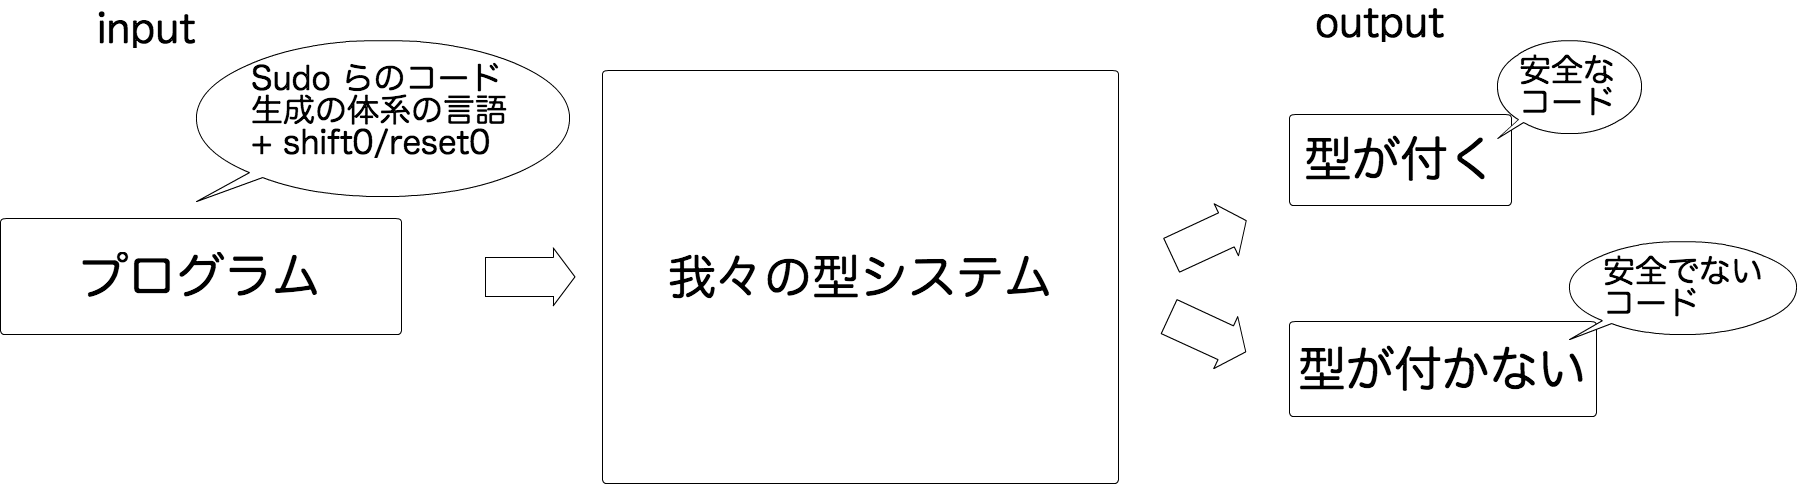
\includegraphics[clip,height=3.2cm]{./img/code_s0r0.png}
    \end{column}
  \end{columns}
\end{frame}

\subsection{多段階let 挿入}
\begin{frame}[fragile]
  \frametitle{多段階let 挿入}
  \begin{align*}
    & \cLet~x_1=\csp{3}~\cIn \\
    & \cLet~x_2=\csp{5}~\cIn \\
    & \magenta{\cLet~y=t~\cIn} \\
    & (x_1~\cPlus~x_2~\cPlus~y)
  \end{align*}

  \pause

  \begin{align*}
    & \red{\cResetz} ~~\cLet~x_1=\csp{3}~\cIn \\
    & \blue{\cResetz} ~~\cLet~x_2=\csp{5}~\cIn \\
    & \blue{\cShiftz}~\blue{k_2}~\to~ \red{\cShiftz}~\red{k_1}~\to~ \magenta{\cLet~y=t~\cIn} \\
    & \cThrow~\red{k_1}~(\cThrow~\blue{k_2}~(x_1~\cPlus~x_2~\cPlus~y))
  \end{align*}
\end{frame}

\begin{frame}
  \frametitle{shift0/reset0 による多段階let挿入}
    \begin{onlyenv}<1>
    \begin{align*}
      & \red{\cResetz} ~~\cLet~x_1=\csp{3}~\cIn \\
      & \blue{\cResetz} ~~\cLet~x_2=\csp{5}~\cIn \\
      & \blue{\cShiftz}~\blue{k_2}~\to~ \red{\cShiftz}~\red{k_1}~\to~ \magenta{\cLet~y=t~\cIn} \\
      & \phantom{=}~~ \cThrow~\red{k_1}~(\cThrow~\blue{k_2}~(x_1~\cPlus~x_2~\cPlus~y))
    \end{align*}
  \end{onlyenv}

  \begin{onlyenv}<2>
    \begin{align*}
      & \red{\cResetz} ~~\cLet~x_1=\csp{3}~\cIn \\
      & \blue{\cResetz} ~~\cLet~x_2=\csp{5}~\cIn \\
      & \blue{\cShiftz}~\blue{k_2}~\to~ \red{\cShiftz}~\red{k_1}~\to~ \magenta{\cLet~y=t~\cIn} \\
      & \cThrow~\red{k_1}~(\cThrow~\blue{k_2}~(x_1~\cPlus~x_2~\cPlus~y))
    \end{align*}
    \begin{align*}
      \red{k_1} &= \cLet~x_1=\csp{3}~\cIn  \\
      \blue{k_2} &= \cLet~x_2=\csp{5}~\cIn  \\
    \end{align*}
  \end{onlyenv}

  \begin{onlyenv}<3>
    \begin{align*}
      & \magenta{\cLet~y=t~\cIn} \\
      & \cThrow~\red{k_1}~(\cThrow~\blue{k_2}~(x_1~\cPlus~x_2~\cPlus~y))
    \end{align*}
    \begin{align*}
      \red{k_1} &= \cLet~x_1=\csp{3}~\cIn  \\
      \blue{k_2} &= \cLet~x_2=\csp{5}~\cIn  \\
    \end{align*}
  \end{onlyenv}

  \begin{onlyenv}<4>
    \begin{align*}
      & \magenta{\cLet~y=t~\cIn} \\
      & \cLet~x_1=\csp{3}~\cIn \\
      & \cLet~x_2=\csp{5}~\cIn \\
      & (x_1~\cPlus~x_2~\cPlus~y)
    \end{align*}
  \end{onlyenv}
\end{frame}

\begin{frame}
  \frametitle{shift0/reset0による多段階let挿入の結果}
  \begin{align*}
    & \cLet~x_1=\csp{3}~\cIn \\
    & \cLet~x_2=\csp{5}~\cIn \\
    & \magenta{\cLet~y=t~\cIn} \\
    & (x_1~\cPlus~x_2~\cPlus~y)
  \end{align*}
  \pause
  \begin{align*}
    & \Rightarrow (\text{shift0/reset0 を付与})\\
  \end{align*}
  \pause
  \begin{align*}
    & \magenta{\cLet~y=t~\cIn} \\
    & \cLet~x_1=\csp{3}~\cIn \\
    & \cLet~x_2=\csp{5}~\cIn \\
    & (x_1~\cPlus~x_2~\cPlus~y)
  \end{align*}
\end{frame}

\subsection{型システム}
\begin{frame}
  % \frametitle{型システムの設計方針}
  \frametitle{変数スコープの利用 by Sudo}
  % スコープが変わるところは,classifier の順序だけで済んでる
  % 合流がある classifier について
  \begin{onlyenv}<1>
    一般的なshift0/reset0 (throw) の式の形
    \begin{align*}
      (\cResetz ~...~ (\cShiftz ~k \to ~...~ (\cThrow ~k ~...~)))
    \end{align*}
  \end{onlyenv}

  \begin{onlyenv}<2>
    \begin{itemize}
    \item $\gamma$は変数のスコープを表す.
    \item その時点で使える自由変数の集合と思ってもらえば良い.
    \item $\gamma$には,包含関係があり,それを $\gamma_0 \ord \gamma_1$ というような順序で表している.
    \item 直感的には$\gamma_1$より$\gamma_0$のほうが使える自由変数が多いという意味である.
    \end{itemize}

    \begin{align*}
      (\cResetz ~\gamma_0~ (\cShiftz ~k \to ~\gamma_1~ (\cThrow ~k ~\gamma_3)))
    \end{align*}
  \end{onlyenv}
\end{frame}

\begin{frame}
  % \frametitle{型システムの設計方針}
  \frametitle{shift0/reset0 によるlet挿入が型安全性を保つ条件}
  % スコープが変わるところは,classifier の順序だけで済んでる
  % 合流がある classifier について
  \begin{onlyenv}<1>
    一般的なshift0/reset0 (throw) の式の形
    \begin{align*}
      (\cResetz ~...~ (\cShiftz ~k \to ~...~ (\cThrow ~k ~...~)))
    \end{align*}
  \end{onlyenv}


  \begin{onlyenv}<2>
    \begin{columns}
      \begin{column}{0.5\textwidth}%% [横幅] 0.2\textwidth = ページ幅の 20 %
        \begin{align*}
          &(\cResetz ~\cLet~ y = e_1 ~\cIn~ \red{...} \\
          &(\cShiftz ~k \to ~\cLet~ x = \red{...} ~\cIn~ \red{...}\\
          &(\cThrow ~k ~\red{...}~)))\\
          &=> \\
          &(\cResetz ~\cLet~ y = e_1 ~\cIn~ \red{\gamma_0} \\
          &(\cShiftz ~\magenta{k} \to ~\cLet~ x = \red{\gamma_1} ~\cIn~ \red{\gamma_2} \\
          &(\cThrow ~\blue{k} ~\red{\gamma_3}~)))
        \end{align*}
      \end{column}

      \begin{column}{0.5\textwidth}%% [横幅] 0.2\textwidth = ページ幅の 20 %
        \center
        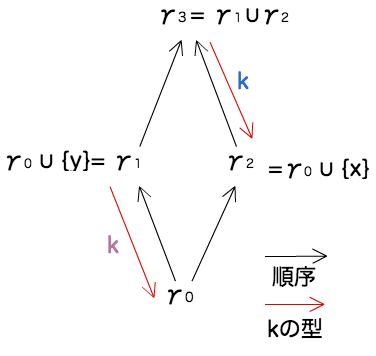
\includegraphics[clip,height=4cm]{./img/index.png}
        \begin{align*}
          \magenta{k} ~:~ \contT{\codeT{\cdot}{\gamma_1}}{\codeT{\cdot}{\gamma_0}}\\
          \blue{k} ~:~  \contT{\codeT{\cdot}{\gamma_3}}{\codeT{\cdot}{\gamma_2}}\\
        \end{align*}
      \end{column}
    \end{columns}
  \end{onlyenv}

\end{frame}


% \begin{frame}
%   \frametitle{Typing rule}
%   \begin{align*}
%     t & ::= \textrm{BasicType} \mid t \to t \mid \codeT{t}{\gamma}
%   \end{align*}

%   Typing rule for code-level lambda:
%   \[
%     \infer[(\gamma_1~\text{is eigen var})]
%     {\Gamma \vdash \cfun{x}{e} ~:~ \codeT{t_1\to t_2}{\gamma}}
%     {\Gamma,~\gamma_1 \ord \gamma,~x:\codeT{t_1}{\gamma_1} \vdash e
%       ~:~ \codeT{t_2}{\gamma_1}}
%   \]

%   Typing rule for code-level let (derived rule):
%   \[
%     \infer[(\gamma_1~\text{is eigen var})]
%     {\Gamma \vdash \clet{x}{e_1}{e_2} ~:~ \codeT{t_2}{\gamma}}
%     {\Gamma \vdash e_1 ~:~ \codeT{t_1}{\gamma}
%       &\Gamma,~\gamma_1 \ord \gamma,~x:\codeT{t_1}{\gamma_1} \vdash
%       e_2 ~:~ \codeT{t_2}{\gamma_1}
%     }
%   \]

%   Typing rule for code-level reset0:
%   \[
%     \infer{\Gamma \vdash \cresetz{e} ~:~ \codeT{t}{\gamma}}
%     {\Gamma \vdash e ~:~ \codeT{t}{\gamma}}
%   \]

%   Typing rule for code-level shift0:
%   \[
%     \infer{\Gamma \vdash \cshiftz{k}{e} ~:~ \codeT{t_1}{\gamma_1}}
%     {\Gamma,~k:\contT{\codeT{t_1}{\gamma_1}}{\codeT{t_0}{\gamma_0}}
%       \vdash e ~:~ \codeT{t_0}{\gamma_0}}
%   \]

%   Typing rule for code-level throw:
%   \[
%     \infer[(\gamma_3~\text{is eigen var})]
%     {\Gamma \vdash \cthrow{k}{e} ~:~ \codeT{t_0}{\gamma_2}}
%     {\Gamma,~k:\contT{\codeT{t_1}{\gamma_1}}{\codeT{t_0}{\gamma_0}},~
%       \gamma_3 \ord \gamma_1,~
%       \gamma_3 \ord \gamma_2
%       \vdash e ~:~ \codeT{t_1}{\gamma_3}
%       & \Gamma \models \gamma_2 \ord \gamma_0
%     }
%   \]
% \end{frame}

\subsection{型付けの例}
\begin{frame}
  \frametitle{型が付く例/付かない例}
  \begin{align*}
    e_1 & = \cResetz ~~\cLet~x_1=\csp{3}~\cIn \\
        & \phantom{=}~~ \cResetz ~~\cLet~x_2=\csp{5}~\cIn \\
        & \phantom{=}~~ \cShiftz~k~\to~ \red{\cLet~y=t~\cIn} \\
        & \phantom{=}~~ \cThrow~k~(x_1~\cPlus~x_2~\cPlus~y)
  \end{align*}

  \pause

  \begin{align*}
    e_1 & \too \cResetz ~~\cLet~x_1=\csp{3}~\cIn \\
        & \phantom{\too}~~ \red{\cLet~y=t~\cIn} \\
        & \phantom{\too}~~ \cResetz ~~\cLet~x_2=\csp{5}~\cIn \\
        & \phantom{\too}~~ (x_1~\cPlus~x_2~\cPlus~y)
  \end{align*}

  \pause
  $t=\csp{7}$ か $t=x_1$ のとき $e_1$ は型が付く

  $t=x_2$ のとき $e_1$ は型が付かない

\end{frame}

\begin{frame}
  \frametitle{型が付く例/付かない例}
  \begin{align*}
    e_2 & = \cResetz ~~\cLet~x_1=\csp{3}~\cIn \\
        & \phantom{=}~~ \cResetz ~~\cLet~x_2=\csp{5}~\cIn \\
        & \phantom{=}~~ \cShiftz~k_2~\to~ \cShiftz~k_1~\to~ \red{\cLet~y=t~\cIn} \\
        & \phantom{=}~~ \cThrow~k_1~(\cThrow~k_2~(x_1~\cPlus~x_2~\cPlus~y))
  \end{align*}

  \pause

  \begin{align*}
    e_2 & \too \red{\cLet~y=t~\cIn} \\
        & \phantom{\too}~~ \cResetz ~~\cLet~x_1=\csp{3}~\cIn \\
        & \phantom{\too}~~ \cResetz ~~\cLet~x_2=\csp{5}~\cIn \\
        & \phantom{\too}~~ (x_1~\cPlus~x_2~\cPlus~y)
  \end{align*}

  \pause
  $t=\csp{7}$ のとき $e_2$ は型が付く

  $t=x_2$ か $t=x_1$ のとき $e_2$ は型が付かない
\end{frame}

\section{まとめと今後}
\begin{frame}
  \frametitle{まとめと今後}
  \begin{itemize}
  % \item コードの言語にshift0 reset0 を組み込んだ言語の設計を行った
  \item コードの型システムに shift0 reset0 を組み込んだ 型システムの設計を行った
  \item その型システムによって型が付く場合と付かない場合の例をみた.
  \item 今後 answer type modification に対応した型システムを設計し,(subject reduction 等の)健全性の証明を行う
  \end{itemize}
\end{frame}

\end{document}

%%% Local Variables:
%%% mode: japanese-latex
%%% TeX-master: t
%%% End:
